\documentclass[aspectratio=169,11pt]{beamer}
\usepackage[T1]{fontenc}
\usepackage{lmodern}
\usepackage{amsmath,amssymb}
\usepackage{booktabs,tabularx,array}
\usepackage{tikz}
\usetikzlibrary{arrows.meta,positioning,calc}

% ---------------------------------------------------------------- look (same as cruise_lab_slides.tex)
\definecolor{ink}{HTML}{1F2328}
\definecolor{muted}{HTML}{6B7280}
\definecolor{flight}{HTML}{2A78D6}
\definecolor{twin}{HTML}{EB6834}
\definecolor{panel}{HTML}{F3F5F8}
\setbeamercolor{normal text}{fg=ink}
\setbeamercolor{frametitle}{fg=ink,bg=white}
\setbeamercolor{structure}{fg=flight}
\setbeamercolor{block title}{fg=white,bg=flight}
\setbeamercolor{block body}{bg=panel}
\setbeamertemplate{navigation symbols}{}
\setbeamertemplate{itemize items}{\color{flight}\textbullet}
\setbeamerfont{frametitle}{size=\Large,series=\bfseries}
\setbeamertemplate{frametitle}{\vspace{0.5em}\insertframetitle\par\vspace{-0.2em}{\color{flight}\rule{2.2cm}{1.5pt}}}
\setbeamertemplate{footline}{\hfill{\color{muted}\scriptsize Cruise Lab: technical write-up \quad \insertframenumber/\inserttotalframenumber}\hspace{1.2em}\vspace{0.6em}}
\newcommand{\obs}[1]{{\color{flight}\textbf{#1}}}
\newcommand{\ctl}[1]{{\color{twin}\textbf{#1}}}
\newcommand{\aside}[1]{{\color{muted}\small #1}}
\newcolumntype{L}{>{\raggedright\arraybackslash}X}

\begin{document}

% ================================================================ 1
\begin{frame}[plain]
  \vspace{2.5em}
  {\Huge\bfseries Cruise Lab}\\[0.6em]
  {\Large Technical write-up: how the anomaly data is generated}\\[1.4em]
  {\color{flight}\rule{3cm}{2pt}}\\[1em]
  Kartik \quad\textbullet\quad IISc \quad\textbullet\quad October 2026\\[2.5em]
  \aside{Process, models, parameters and checks. No result plots.}
\end{frame}

% ================================================================ 2
\begin{frame}{Goal and scope}
  \begin{itemize}\setlength\itemsep{0.7em}
    \item \textbf{Goal:} labelled B747 cruise flights for anomaly-detection research, where each fault's type, location, size, onset and duration are known exactly.
    \item \textbf{Tool:} JSBSim 1.3.1 (open-source 6-DOF flight dynamics, FlightGear's physics), driven from Python, headless.
    \item \textbf{Scope:} cruise phase only, 25--35 min per flight, one anomaly per anomalous flight.
    \item \textbf{Two anomaly families:} \obs{observation} (sensor reading corrupted before the autopilot) and \ctl{control} (command corrupted after the autopilot). 14 types in total.
    \item \textbf{Ground truth:} each anomalous flight has a \textbf{normal twin} (same seed, no anomaly).
    \item \textbf{Status:} data generation only; detector training is the next phase.
  \end{itemize}
\end{frame}

% ================================================================ 3
\begin{frame}{The generation pipeline (one flight)}
  \centering
  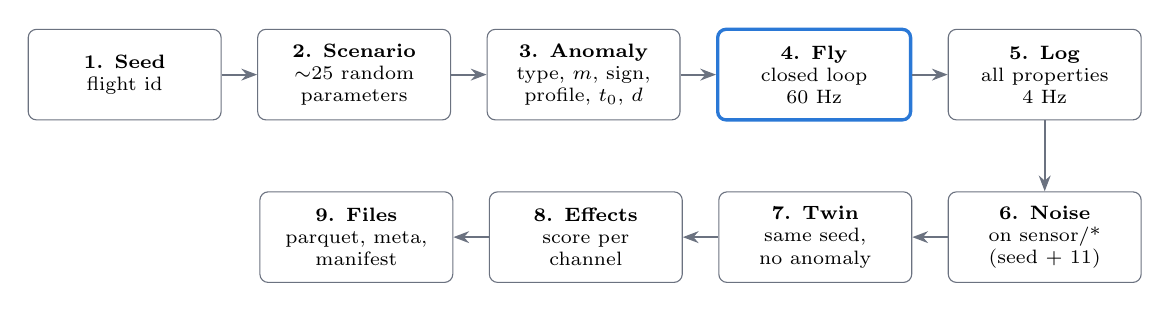
\begin{tikzpicture}[
      st/.style={draw=muted, rounded corners=3pt, minimum width=2.45cm, minimum height=1.15cm, align=center, font=\scriptsize},
      arr/.style={-{Stealth[length=2mm]}, draw=muted, thick}]
    \node[st] (seed) {\textbf{1. Seed}\\flight id};
    \node[st, right=0.45cm of seed] (scen) {\textbf{2. Scenario}\\$\sim$25 random\\parameters};
    \node[st, right=0.45cm of scen] (anom) {\textbf{3. Anomaly}\\type, $m$, sign,\\profile, $t_0$, $d$};
    \node[st, right=0.45cm of anom, draw=flight, very thick] (fly) {\textbf{4. Fly}\\closed loop\\60 Hz};
    \node[st, right=0.45cm of fly] (log) {\textbf{5. Log}\\all properties\\4 Hz};
    \node[st, below=0.9cm of log] (noise) {\textbf{6. Noise}\\on sensor/*\\(seed + 11)};
    \node[st, left=0.45cm of noise] (twin) {\textbf{7. Twin}\\same seed,\\no anomaly};
    \node[st, left=0.45cm of twin] (eff) {\textbf{8. Effects}\\score per\\channel};
    \node[st, left=0.45cm of eff] (out) {\textbf{9. Files}\\parquet, meta,\\manifest};
    \draw[arr] (seed) -- (scen); \draw[arr] (scen) -- (anom); \draw[arr] (anom) -- (fly);
    \draw[arr] (fly) -- (log); \draw[arr] (log) -- (noise); \draw[arr] (noise) -- (twin);
    \draw[arr] (twin) -- (eff); \draw[arr] (eff) -- (out);
  \end{tikzpicture}
  \vspace{1em}

  \small
  \begin{tabularx}{\textwidth}{@{}l L@{}}
    \toprule
    Code & \texttt{lab/scenario.py} (2) \textbullet{} \texttt{anomalies.py} (3) \textbullet{} \texttt{simulate.py} (4--6) \textbullet{} \texttt{generate.py} (7--9) \\
    Run & \texttt{python -m lab.generate -{}-preset demo|catalog|random}, 6 worker processes \\
    Speed & $\approx$ 7 s per 30-min flight ($\approx$ 250$\times$ real time) \\
    \bottomrule
  \end{tabularx}
\end{frame}

% ================================================================ 4
\begin{frame}{Closed loop: where the anomaly enters}
  \centering
  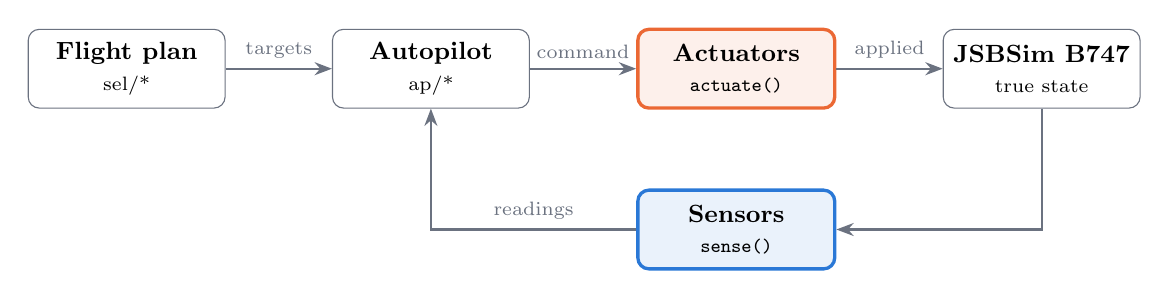
\begin{tikzpicture}[
      box/.style={draw=muted, rounded corners=4pt, minimum width=2.5cm, minimum height=1.0cm, align=center, font=\small},
      arr/.style={-{Stealth[length=2.2mm]}, draw=muted, thick},
      lab/.style={font=\scriptsize, text=muted}]
    \node[box] (plan) {\textbf{Flight plan}\\\scriptsize sel/*};
    \node[box, right=1.35cm of plan] (ap) {\textbf{Autopilot}\\\scriptsize ap/*};
    \node[box, right=1.35cm of ap, draw=twin, fill=twin!10, very thick] (act) {\textbf{Actuators}\\\scriptsize \texttt{actuate()}};
    \node[box, right=1.35cm of act] (fdm) {\textbf{JSBSim B747}\\\scriptsize true state};
    \node[box, below=1.0cm of act, draw=flight, fill=flight!10, very thick] (sen) {\textbf{Sensors}\\\scriptsize \texttt{sense()}};
    \draw[arr] (plan) -- node[lab, above] {targets} (ap);
    \draw[arr] (ap) -- node[lab, above] {command} (act);
    \draw[arr] (act) -- node[lab, above] {applied} (fdm);
    \draw[arr] (fdm.south) |- (sen.east);
    \draw[arr] (sen.west) -| node[lab, pos=0.25, above] {readings} (ap.south);
  \end{tikzpicture}
  \vspace{0.6em}

  \small
  \textbf{Each 1/60 s:} plan $\rightarrow$ \obs{sense} 9 readings (ALT CAS VS PITCH ROLL HDG BETA Q P) $\rightarrow$ autopilot $\rightarrow$ \ctl{actuate} elevator, aileron, rudder, 4 throttles $\rightarrow$ JSBSim step.
  \vspace{0.4em}

  \begin{tabularx}{\textwidth}{@{}L L@{}}
    \toprule
    \obs{Observation}: autopilot acts correctly on a wrong reading $\Rightarrow$ the aircraft really leaves its target; the faulty sensor looks normal. &
    \ctl{Control}: autopilot acts correctly on true readings, but its command is altered $\Rightarrow$ it sees a wrong response and compensates. \\
    \bottomrule
  \end{tabularx}
\end{frame}

% ================================================================ 5
\begin{frame}{Aircraft, scenario and autopilot}
  \begin{columns}[T]
    \begin{column}{0.47\textwidth}
      \textbf{Aircraft} {\color{muted}\scriptsize (\texttt{aircraft.py})}
      \begin{itemize}\scriptsize
        \item JSBSim B747 + payload point mass; tanks 10.9 $\rightarrow$ 25 klb
        \item trimmed at cruise, then small random attitude/rate disturbance
        \item elevator sign measured at start-up, not assumed
      \end{itemize}
      \textbf{Normal variability} {\color{muted}\scriptsize (\texttt{scenario.py})}
      \begin{itemize}\scriptsize
        \item altitude 28--34 kft, Mach 0.705--0.735, heading 0--360$^\circ$
        \item 0--3 turns, 30\,\% step climb, 30\,\% Mach change
        \item wind 0--50 kt, ISA $\pm$ N(0, 5)\,$^\circ$C, Dryden turbulence
        \item payload 20--120 klb, fuel 60--90\,\%, AP gains $\times$U(0.85, 1.15)
      \end{itemize}
    \end{column}
    \begin{column}{0.5\textwidth}
      \textbf{Autopilot} {\color{muted}\scriptsize (\texttt{autopilot.py}, 60 Hz, reads sensed values only)}
      \begin{itemize}\scriptsize
        \item altitude $\rightarrow$ VS cmd $\rightarrow$ pitch (PI) $\rightarrow$ elevator (P + pitch-rate damping)
        \item CAS $\rightarrow$ throttle PID, anti-windup, slew 0.055/s, one command to 4 engines
        \item heading $\rightarrow$ bank ($\pm$25$^\circ$) $\rightarrow$ aileron (P + roll-rate damping)
        \item sideslip $\rightarrow$ rudder (PI)
      \end{itemize}
      \vspace{0.2em}
      {\color{muted}\scriptsize Custom autopilot because every input must pass through \texttt{sense()}. Gains from the verified v2 notebooks.}\\[0.4em]
      \textbf{Hard normals} {\color{muted}\scriptsize (labelled normal, test false alarms)}\\
      {\scriptsize moderate turbulence, 70--100 kt wind, hot / cold day ($\pm$15--22\,$^\circ$C), heavy (140--160 klb)}
    \end{column}
  \end{columns}
\end{frame}

% ================================================================ 6
\begin{frame}{The anomaly model: one pattern}
  \vspace{-0.6em}
  \[
    \underbrace{\text{reading}}_{\text{to autopilot}} = \text{true} + \text{sign}\cdot m\cdot g(t)
    \qquad\qquad
    \underbrace{\text{applied}}_{\text{to aircraft}} = \text{command} + \text{sign}\cdot m\cdot g(t)
  \]
  \small
  \begin{tabularx}{\textwidth}{@{}l L@{}}
    \toprule
    \textbf{true / command} & simulator's real value / autopilot's output at time $t$ \\
    \textbf{$m$} & magnitude, always $> 0$, fixed for the whole flight; unit of the target (ft, kt, $^\circ$, command units, fraction) \\
    \textbf{sign} & $\pm1$ with equal probability: direction of the error \\
    \textbf{$g(t)$} & envelope in $[0,1]$: 0 outside $[t_0, t_{end})$; step = 1, ramp = $(t-t_0)/(t_{end}-t_0)$, intermittent = 1 in bursts \\
    \textbf{units} & surfaces $-1\dots+1$ ($-1$ = full nose-up elevator here, $\approx$20$^\circ$ per unit); throttle $0\dots1$ \\
    \bottomrule
  \end{tabularx}
  \vspace{0.3em}

  \small\textbf{Example (C100, elevator bias):} $m = 0.0617$ ($\approx$1.2$^\circ$), sign $-$, step, 501.5--612.1 s $\Rightarrow$ applied $=$ command $- 0.0617$.
  The autopilot raises its command by $+0.062$ to cancel it: the signature is \textbf{command $\neq$ applied}.
\end{frame}

% ================================================================ 7
\begin{frame}{Catalogue: 14 types}
  \scriptsize
  \begin{columns}[T]
    \begin{column}{0.49\textwidth}
      \obs{Observation} (9 sensed variables)\\[0.3em]
      \begin{tabularx}{\linewidth}{@{}l L l@{}}
        \toprule
        Type & Injection & Max \\
        \midrule
        bias & true $+ s\,m\,g$ & 900 s \\
        drift & true $+ s\,2m\,\frac{t-t_0}{t_{end}-t_0}$ & 900 s \\
        stuck & true$(t_0)$ frozen & 180 s \\
        noise & true $+\,\mathcal N(0,(m/2)^2)$ & 600 s \\
        spikes & true $\pm 3m$, 0.25--1 s, $\sim$4/min & 600 s \\
        pitot blockage & $p_t$ frozen, CAS from $p_t^*-p_s(h)$ & 300 s \\
        \bottomrule
      \end{tabularx}
    \end{column}
    \begin{column}{0.49\textwidth}
      \ctl{Control} (elevator, aileron, rudder, 1 engine)\\[0.3em]
      \begin{tabularx}{\linewidth}{@{}l L l@{}}
        \toprule
        Type & Injection & Max \\
        \midrule
        surface bias & $u + s\,m\,g$ & 900 s \\
        surface stuck & $u(t_0)$ frozen & 120 s elev. \\
        loss of effect. & $u(1 - m\,g)$ & 900 s \\
        oscillation & $u + m\,g\sin 2\pi f(t-t_0)$ & 600 s \\
        runaway & $u + s\,m\min(1,\frac{t-t_0}{30})$ & 300 s \\
        thrust loss & $u_e(1 - m\,g)$ & 900 s \\
        lever stuck & $u_e(t_0)$ frozen & 900 s \\
        lever bias & $u_e + s\,m\,g$ & 900 s \\
        \bottomrule
      \end{tabularx}
    \end{column}
  \end{columns}
  \vspace{0.8em}

  \small Draw order (own RNG, seed + 7): group $\rightarrow$ type (weights) $\rightarrow$ variable $\rightarrow$ severity $\rightarrow m$ $\rightarrow$ profile $\rightarrow t_0 \rightarrow d \rightarrow$ sign.
  Stuck and pitot types have no $m$.
\end{frame}

% ================================================================ 8
\begin{frame}{Magnitude: lo, hi and severity}
  \begin{columns}[T]
    \begin{column}{0.48\textwidth}
      \vspace{-0.8em}
      \[ m = lo\left(\frac{hi}{lo}\right)^{s},\qquad s \sim U(0,1) \]
      \footnotesize
      \begin{itemize}\setlength\itemsep{0.3em}
        \item \textbf{lo} = weakest allowed fault $\approx$ a few $\times$ normal noise/turbulence (hard)
        \item \textbf{hi} = strongest: clearly abnormal, still flyable (easy, not trivial)
        \item \textbf{severity} $s$ = position between them on a log scale; demo uses $s = 0.7$
        \item lo, hi are offsets, not positions on the $-1\dots1$ scale
      \end{itemize}
      \vspace{0.1em}
      \scriptsize
      \begin{tabularx}{\linewidth}{@{}L r r@{}}
        \toprule
        Example & lo & hi \\
        \midrule
        ALT bias & 50 ft & 400 ft \\
        CAS bias & 3 kt & 15 kt \\
        elevator bias & 0.02 & 0.10 \\
        thrust loss & 5\,\% & 40\,\% \\
        \bottomrule
      \end{tabularx}
    \end{column}
    \begin{column}{0.49\textwidth}
      \textbf{Why log-uniform, not linear} {\color{muted}\scriptsize (ALT, 50--400 ft)}\\[0.2em]
      \footnotesize
      \begin{tabularx}{\linewidth}{@{}L r r@{}}
        \toprule
        Range & Linear & Log \\
        \midrule
        50--100 ft (hard) & 14\,\% & 33\,\% \\
        100--200 ft & 29\,\% & 33\,\% \\
        200--400 ft (easy) & 57\,\% & 33\,\% \\
        \bottomrule
      \end{tabularx}
      \vspace{0.4em}
      \begin{itemize}\footnotesize
        \item detectability depends on the \emph{ratio} to noise, so each doubling gets equal weight
        \item linear draws favour large, easy faults and inflate detector scores
        \item same severity means the same relative strength for every variable
      \end{itemize}
      {\color{muted}\scriptsize lo/hi are engineering judgement. Planned: calibrate so lo gives effect score $\approx$1, hi $\approx$10.}
    \end{column}
  \end{columns}
\end{frame}

% ================================================================ 9
\begin{frame}{Timing: onset, duration, profile}
  \begin{columns}[T]
    \begin{column}{0.5\textwidth}
      \[ t_0 \sim U(300\,\mathrm{s},\ T - 420\,\mathrm{s}) \]
      \[ d = \mathrm{clip}\big(e^{\mathcal N(\ln 300,\,0.6^2)},\ 60,\ \min(d_{max}, T-120-t_0)\big) \]
      \small
      \begin{itemize}
        \item first 300 s hold the start-up transient
        \item $\geq$ 120 s recovery tail after every fault
        \item uniform onset: no fixed time to learn
        \item log-normal: median 5 min, middle 68\,\% $\approx$ 2.7--9 min
        \item $d_{max}$ per type keeps dangerous faults short
      \end{itemize}
    \end{column}
    \begin{column}{0.47\textwidth}
      \textbf{Profiles} \aside{(weights 0.5 / 0.3 / 0.2)}
      \begin{itemize}\small\setlength\itemsep{0.4em}
        \item \textbf{step}: full fault at onset (jam, sudden failure)
        \item \textbf{ramp}: grows 0 $\rightarrow$ full over the window (degradation)
        \item \textbf{intermittent}: bursts ON 20--60 s, OFF 30--120 s; window $\geq$ 300 s (loose connector)
      \end{itemize}
      \vspace{0.4em}
      \textbf{Labels} (per 4 Hz row)
      \[ \mathrm{label} = \mathbf 1[t_0 \le t < t_{end}] \ \wedge\ \text{in a burst} \]
      \aside{Recovery after the end is labelled 0.}
    \end{column}
  \end{columns}
\end{frame}

% ================================================================ 10
\begin{frame}{Safety checks and limits}
  \small
  \begin{tabularx}{\textwidth}{@{}l L@{}}
    \toprule
    \textbf{In place} & \\
    \midrule
    magnitude bounds & $m$ always within [lo, hi] for its type and variable \\
    duration caps & elevator stuck $\le$ 120 s, pitot $\le$ 300 s, others $\le$ 600--900 s \\
    onset / tail & no fault before 300 s; $\ge$ 120 s after the end \\
    command clipping & after the anomaly: surfaces to $[-1, 1]$, throttle to $[0, 1]$ \\
    autopilot limits & pitch $-8\dots12^\circ$, bank $\pm25^\circ$, rudder $\pm0.4$, throttle $\ge 0.18$, VS limited \\
    pitot floor & impact pressure $\ge 0$, indicated CAS $\ge$ 30 kt \\
    crash handling & JSBSim stop $\Rightarrow$ error, flight not saved \\
    bad values & $|x| > 10^{15}$ stored as NaN; \texttt{gear/}, \texttt{ground/} excluded (garbage in the air) \\
    \midrule
    \textbf{Not yet} & no envelope check after the flight (stall $\alpha$, overspeed, bank, altitude loss) \\
    \bottomrule
  \end{tabularx}
  \vspace{0.6em}

  \aside{In the demo set the largest excursion was $\approx$380 ft (elevator stuck, C101); no clipping was reached in cruise.}
\end{frame}

% ================================================================ 11
\begin{frame}{Logging, noise and the normal twin}
  \begin{columns}[T]
    \begin{column}{0.48\textwidth}
      \textbf{Logged at 4 Hz} \aside{($\approx$680 channels, 329 change)}
      \begin{itemize}\footnotesize
        \item \texttt{sensor/*}: autopilot readings (+ anomaly + noise), TLA 1--4
        \item \texttt{ap/*}: commands \emph{before} control anomaly
        \item \texttt{sel/*}: flight plan; \texttt{derived/egt}: EGT law
        \item every JSBSim property: the \emph{true} state
      \end{itemize}
      \textbf{Measurement noise} \aside{(Gaussian, logs only)}
      \begin{itemize}\footnotesize
        \item ALT 10 ft, CAS 0.5 kt, VS 30 fpm, attitude 0.05$^\circ$, rates 0.02$^\circ$/s
      \end{itemize}
      \textbf{Files}: Parquet float32 + zstd ($\approx$12 MB/flight), \texttt{meta/<id>.json}, \texttt{manifest.json}
    \end{column}
    \begin{column}{0.49\textwidth}
      \textbf{Normal twin}
      \begin{itemize}\footnotesize
        \item same seed, weather, turbulence and noise; no anomaly
        \item separate seeded streams: scenario (seed), anomaly (+7), noise (+11), anomaly noise (+99), turbulence
        \item removing the anomaly changes nothing else
        \item verified: max $|$flight $-$ twin$|$ before onset $=$ \textbf{0}, all 16 demo twins
      \end{itemize}
      \textbf{Effect score} \aside{(verification, not detection)}
      \[ \mathrm{score}_c = \max_{t\ge t_0}\frac{|x_c - y_c|}{\max(\mathrm{std}\,y_c,\ 10^{-3}|\bar y_c|,\ 0.05\,\mathrm{std}\,x_c)} \]
      \footnotesize strong $\ge$ 3, moderate $\ge$ 1, weak $\ge$ 0.25
    \end{column}
  \end{columns}
\end{frame}

% ================================================================ 12
\begin{frame}{Limitations and next steps}
  \begin{columns}[T]
    \begin{column}{0.48\textwidth}
      \textbf{Limitations}
      \begin{itemize}\footnotesize\setlength\itemsep{0.3em}
        \item table-based aero, simplified turbine model
        \item simple autopilot: no FMS modes, protection or pilot
        \item noise added after the loop, not seen by the autopilot
        \item one sensor per variable, no redundancy
        \item no quantization, mixed rates or dropouts yet
        \item cruise only, one fault per flight
        \item lo/hi and noise levels are judgement, not statistics
      \end{itemize}
    \end{column}
    \begin{column}{0.48\textwidth}
      \textbf{Next steps}
      \begin{enumerate}\footnotesize\setlength\itemsep{0.3em}
        \item envelope check after each flight
        \item calibrate lo/hi from effect scores
        \item catalogue + random sets with train / val / test splits
        \item recorder realism: quantization, rates, dropouts
        \item leakage check: simple thresholds must not catch all
        \item climb/descent, engine-performance faults
        \item then detectors: PR-AUC, false alarms per flight, delay
      \end{enumerate}
    \end{column}
  \end{columns}
\end{frame}

\end{document}
